% !TEX root = template.tex

\section{Related Work}
\label{sec:related_work}

Activity recognition is a field evolving for more than twenty years, it started from very simple motion recognition and it gets more complex over the years.
As just said, the classical approach to this problem is with feature extraction techniques.
In these solutions, ad-hoc features are extracted from the dataset, reducing the dimension of each signals from the recorded sample to a feature vector.
In this way features can be classified using several classifiers to obtain an accurate prediction.

\begin{figure}[!ht]
  \centering
  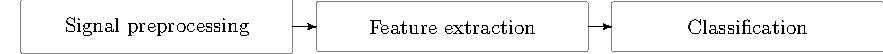
\includegraphics[width=\linewidth]{feature_extraction}
  \caption{Processing pipeline for feature extraction techniques}
  \label{fig:feature_extraction}
\end{figure}

The main processing pipeline used from these solutions is reported in \fig{fig:feature_extraction}.
The most used classifiers for feature extraction are Decision Trees, \gls{svm}, K-nearest neighbors and Naive Bayes although a lot of different classifiers can be used \cite{Ravi05}.

Features can be extracted either from a single sensor or from a large set of sensors, the first solution suffers an high computational complexity while the second is computational easier but certainly less portable and can create issues due to redundancy of the information.
In \cite{Laerhoven02} they collect data from 30 sensors positioned around the body and they classify features extracted from these data with a clustering algorithm. They chose to collect all the data in a central processing unit to perform a centralized classification. This approach suffers however an high cost and an high complexity to limit redundancy in the data.
Varkey et al.'s research, uses only two accelerometer sensors placed at the wrist and ankle \cite{Varkey2012}. They collected data and they predict 6 different activities using an \gls{svm} as classifier, reaching an high accuracy.

The problem of this technique is the strong data dependence even if it gets a good accuracy.

To overcome this lack of the classical \gls{ars}, deep learning is used in several ways.
In \cite{Guenterberg09} an \gls{hmm} is used on data collected by 8 sensors. They firstly compute feature extraction on the data collected from each sensor in a distributed manner, then feature vectors are given in input to the \gls{hmm} that classifies the feature vectors in the activity labels.
In \cite{Chikhaoui17} the authors perform a matrix factorization for dimensionality reduction and deep learning algorithm to automatically learn suitable features.
In this work, they reduce the dimension of the dataset using matrix factorization and they elaborate the results in a \gls{nn}. The output of the \gls{nn} is a feature vector. Finally the activity is predicted classifying the feature vector with a Softmax classifier.
The accuracy is quite good since they avoid hand-crafted features, but they still rely on features extracted from data.

The key to implement an adaptable and reliable algorithm to classify human activities is the use of deep learning without extracting features at all.
A comparison between three different deep learning algorithms is made in \cite{Xu2017}. They collected data from one single sensor and they predicted activities using \gls{dt}, \gls{ann} and \gls{rf}. They stated that \gls{rf} performs better than the other two, with an accuracy between $75 \%$ and $90 \%$ depending on the activity.

Milenkoski et al. use instead \gls{lstm} networks, a specific type of \gls{rnn}, to perform activity prediction in real time on smartphones.
They learn the model using a previously collected dataset to subsequently apply it to new raw data recorded from a smartphone. The reached accuracy is variable between $50\%$, for the most difficult activities to recognize, and $100\%$ for the easiest. The overall accuracy is $88\%$ for the data acquired and pre-processed in laboratory and $82\%$ for the real time prediction \cite{Milenkoski18}.

An interesting solution is the application of \gls{cnn} in the activity recognition field.
In \cite{Panwar17} a \gls{cnn} is used to predict activities using data recorded by a tri-axis accelerometer sensor. They tried to predict very specific activities such as \textit{Fetch cup from desk} or \textit{Pour milk into cup} using a \gls{cnn} made by 3 convolutional layers, one max-pooling layer and a fully connected layer, using a Softmax function to the output of the network.
This application has a recognition rate of $99.8\%$ although is not thought for real time prediction.

The goal of the next sections of this work is to combine a \gls{cnn} architecture with a real time prediction model, to prove that this approach gives results comparable or better than the ones showed in \cite{Korbinian}.